\section{Chứng minh định lý}
$(\Rightarrow)$  Nếu đồ thị $G$ chứa đồ thị con là đồ thị phân chia của $K_5$ hoặc $K_{3,3}$ thì $G$ không phẳng. \\

\begin{proof}
    Ta có:
    \begin{itemize}
        \item Đồ thị phân chia của đồ thị không phẳng thì không phẳng (theo \hyperref[lem:subp]{bổ đề 2})

        \item Nếu một đồ thị con của dồ thị không phẳng thì đồ thị đó không phẳng (theo \hyperref[lem:plnp]{bổ đề 1})
    \end{itemize}
    $\Rightarrow$ Nếu một đồ thị con của đồ thị $G$ là đồ thị phân chia của đồ thị không phẳng thì $G$ không phẳng
    \begin{lemma}
        $K_{3,3}$ không phẳng
    \end{lemma}

    \begin{proof}
        Chúng ta sẽ chứng minh bằng phản chứng.

        Giả sử tồn tại một biểu diễn phẳng của $K_{3,3}$.

        Với $K_{3,3}$, có $\nu = 6, \epsilon = 9$, từ \hyperref[thr:euler]{công thức Euler} ta có:
        \begin{figure}[H]
            \begin{minipage}{0.4\textwidth}
                \begin{eqnarray*}
                    \nu-\epsilon+\phi& = &2 \\
                    6-\epsilon+\phi& = & 2\\
                    6-9+\phi& = & 2\\
                    \phi& = & 5\\
                \end{eqnarray*}
            \end{minipage}
            \hfill
            \begin{minipage}{0.4\textwidth}
                \centering
                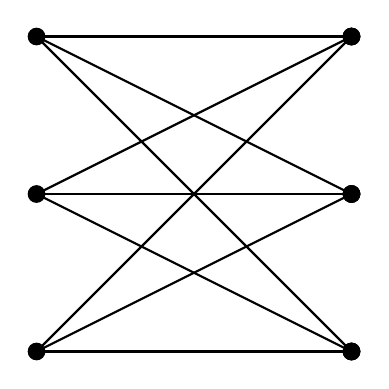
\begin{tikzpicture}
                    \foreach \x/\y in {0/1, 0/3, 0/5} {
                            \filldraw[black] (\x,\y) circle (3pt);
                            \foreach \z/\t in {4/1, 4/3, 4/5} {
                                    \filldraw[black] (\z,\t) circle (3pt);
                                    \draw[black, thick] (\x,\y) -- (\z,\t);
                                }
                        }
                \end{tikzpicture}
            \end{minipage}
        \end{figure}
        Trong đồ thị phân đôi đơn, chiều dài nhỏ nhất của chu trình là 4, nghĩa là với mọi $f \in F(K_{3,3})$
        \begin{eqnarray*}
            deg(f)& \geq &4 \\
            \Rightarrow \sum_{f \in F(K_{3,3})}deg(f)& \geq & 4\phi
        \end{eqnarray*}
        Lại có, từ \hyperref[thr:v2e]{định lý 1}:
        \begin{center}
            \begin{tabular}{ c c c c }
                              & $\displaystyle \sum_{f \in F(K_{3,3})}deg(f)$ & $=$    & $2\epsilon$  \\
                $\Rightarrow$ & $2\epsilon $                                  & $\geq$ & $4\phi$      \\
                $\Rightarrow$ & $2 \times 9$                                  & $\geq$ & $4 \times 5$
            \end{tabular}
        \end{center}
        Vô lý.
    \end{proof}

    \begin{lemma}
        $K_5$ không phẳng
    \end{lemma}
    \begin{proof}
        Giả sử tồn tại một biểu diễn phẳng của $K_5$.

        Với $K_5$, có $\nu = 5, \epsilon = 10$, từ \hyperref[thr:euler]{công thức Euler} ta có:
        \begin{figure}[H]
            \begin{minipage}{0.4\textwidth}
                \begin{eqnarray*}
                    \nu-\epsilon+\phi& = &2 \\
                    5-\epsilon+\phi& = & 2\\
                    5-10+\phi& = & 2\\
                    \phi& = & 7\\
                \end{eqnarray*}
            \end{minipage}
            \hfill
            \begin{minipage}{0.4\textwidth}
                \centering
                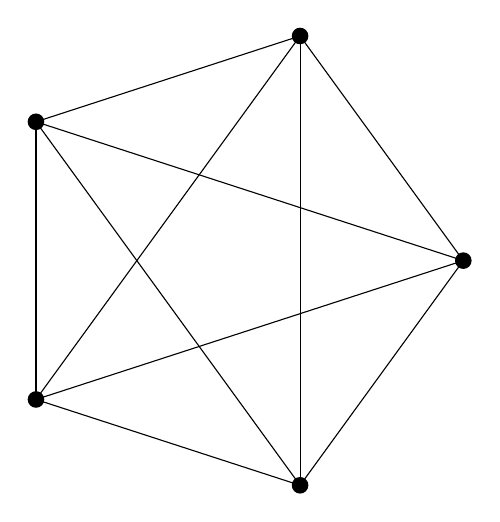
\begin{tikzpicture}
                    \foreach \i in {1, 2, 3, 4, 5}
                    \fill[black] (\i*360/5:3) coordinate (5\i) circle(3 pt)
                    \ifnum \i>1 foreach \j in {\i,...,1}{(5\i) edge (5\j)} \fi;
                \end{tikzpicture}
            \end{minipage}
        \end{figure}
        Trong đồ thị đầy đủ, chiều dài nhỏ nhất của chu trình là 3, nghĩa là với mọi $f \in F(K_5)$
        \begin{eqnarray*}
            deg(f)& \geq &3 \\
            \Rightarrow \sum_{f \in F(K_5)}deg(f)& \geq & 3\phi
        \end{eqnarray*}
        Lại có, từ \hyperref[thr:v2e]{định lý 1}:
        \begin{center}
            \begin{tabular}{ c c c c }
                              & $\displaystyle \sum_{f \in F(K_5)}deg(f)$ & $=$    & $2\epsilon$  \\
                $\Rightarrow$ & $2\epsilon $                              & $\geq$ & $3\phi$      \\
                $\Rightarrow$ & $2 \times 10$                             & $\geq$ & $3 \times 7$
            \end{tabular}
        \end{center}
        Vô lý.
    \end{proof}
    \begin{recap}
    \end{recap}
    $K_5$ và $K_{3,3}$ là không phẳng

    $\Rightarrow$ Tất cả các đồ thị phân chia của chúng đều không phẳng.

    $\Rightarrow$ Nếu đồ thị $G$ chứa đồ thị con là đồ thị phân chia của $K_5$ hoặc $K_{3,3}$ thì G không phẳng. \\

\end{proof}
$(\Leftarrow)$ Nếu đồ thị $G$ không phẳng thì $G$ chứa đồ thị phân chia của $K_5$ hoặc $K_{3,3}$
\begin{proof}
    Giả sử tồn tại đồ thị không phẳng mà không chứa đồ thị con là đồ thị phân chia của $K_5$ và $K_{3,3}$.

    Trong những đồ thị không phẳng không chứa đồ thị con là đồ thị phân chia của $K_5$ và $K_{3,3}$, giả sử $G$ là đồ thị có \textit{ít cạnh nhất}.
    Khi loại bỏ một cạnh bất kì của $G$ thì ta được đồ thị \textit{phẳng}.

    Giả sử $G$ có nhiều thành phần liên thông, dễ thấy $G$ phải có một thành phần liên thông không phẳng. Gọi thành phần liên thông đó là $K$.
    Rõ ràng $\epsilon(K) \leq \epsilon(G)$ và $K$ không chứa đồ thị phân chia của $K_5$ và $K_{3,3}$. Khi $K$ ít cạnh hơn $G$, $G$ sẽ không phải đồ thị \textit{ít cạnh nhất}, mâu thuẫn, do đó $\epsilon(K) = \epsilon(G)$
    và các thành phần liên thông khác $K$ của $G$ đều chỉ gồm đỉnh cô lập. Không mất tính tổng quát, giả sử $G$ liên thông.

    \begin{enumerate}
        \item $G$ là 2-liên thông
              \begin{proof}
                  \begin{figure}[H]
                      \centering
                      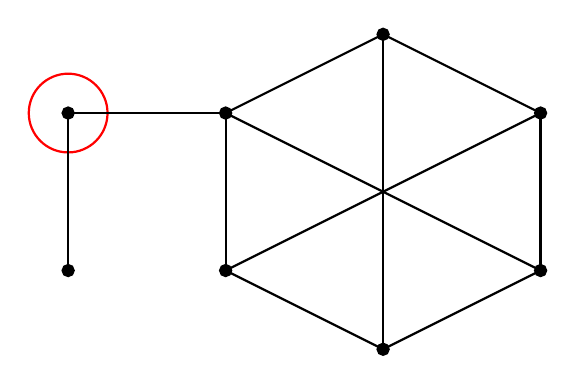
\begin{tikzpicture}
                          \draw[red, thick] (-2,3) circle (0.5);
                          \foreach \x/\y in {0/1, 2/0, 4/1, 0/3, 4/3, 2/4} {
                                  \filldraw[black, thick] (\x,\y) circle (2pt);
                                  \draw[black, thick] (2,2) -- (\x,\y);
                              }
                          \filldraw[black, thick] (-2,3) circle (2pt);
                          \filldraw[black, thick] (-2,1) circle (2pt);

                          \draw[black, thick] (0,1) -- (2,0);
                          \draw[black, thick] (2,0) -- (4,1);
                          \draw[black, thick] (4,1) -- (4,3);
                          \draw[black, thick] (0,3) -- (0,1);
                          \draw[black, thick] (4,3) -- (2,4);
                          \draw[black, thick] (2,4) -- (0,3);

                          \draw[black, thick] (-2,1) -- (-2,3);
                          \draw[black, thick] (-2,3) -- (0,3);

                      \end{tikzpicture}
                  \end{figure}
                  %   Đầu tiên, ta chỉ ra $G$ 1-liên thông (liên thông). Giả sử $G$ không liên thông, và không phẳng.
                  %   Vì $G$ là đồ thị không phẳng \textit{ít cạnh nhất} nên các thành phần của nó là phẳng. Không mất tính tổng quát, giả sử G có 2 thành phần liên thông là $G_1$ và $G_2$.
                  %   Bởi vì $G_1$ và $G_2$ cùng phẳng, ta có thể thêm biểu diễn phẳng của $G_1$ vào một trong các diện biểu diễn phẳng của $G_2$ (ví dụ diện vô hạn), cho ta biểu diễn phẳng của $G$. Vô lý.

                  Vì $G$ liên thông nên $\kappa(G) \geq 1$. Giả sử $\kappa(G) = 1$, theo định nghĩa, tồn tại đỉnh $v$ sao cho $G -v$ không liên thông.
                  Không mất tính tổng quát, giả sử $G-v$ có 2 thành phần liên thông $H_1$ và $H_2$.
                  Ta có $H_1 \cup v$ và $H_2 \cup v$ đều phẳng vì chúng là đồ thị con của $G$ và ít cạnh hơn $G$, đồng thời không chứa đồ thị phân chia của $K_5$ và $K_{3,3}$.
                  Trong biểu diễn phẳng của chúng, ta có thể tìm một diện $f$ mà biên chứa đỉnh $v$.
                  Với phép chiếu lập thể, ta có thể thu được biểu diễn phẳng của $H_1 \cup v$ và $H_2 \cup v$ mà $v$ nằm trên đường biên của diện không bị chặn.
                  Bằng cách đặt điểm ở vô cùng.
                  Sau đó, ta gộp $H_1 \cup v$ và $H_2 \cup v$ bằng cách hợp nhất $v$ và thu được một biểu diễn phẳng của G. Vô lý.
                  \begin{figure}[H]
                      \centering
                      \begin{tikzpicture}[line join=round, line cap=round, >=stealth]%Hinh nón
                          \def\a{1}% Bán trục lớn
                          \def\b{\a/3}% Bán trục bé
                          \pgfmathsetmacro{\h}{sqrt(3)*\a}% Chiều cao
                          \pgfmathsetmacro{\t}{asin(\b/\h)}
                          \shade[ball color=cyan,opacity=0.65](-\h*0.75,0.15*\h)circle(\h);
                          \begin{scope}[xslant=-0.9,magenta]
                              \coordinate (M) at ({\a*cos(\t)}, {\b*sin(\t)});
                              \coordinate (N) at ({-\a*cos(\t)}, {\b*sin(\t)});
                              \path(0,0)coordinate(O)(\a,0)coordinate(A)(-\a,0)coordinate(B);
                              \path (0,\h)coordinate(S)(intersection of A--B and S--N)coordinate(N');
                              \pgfmathsetmacro{\s}{0.5*atan((\h-\b*sin(\t))/(\a*cos(\t)))}
                              \path([rotate around ={{\s}:(N')}]A)coordinate(K)(intersection of N'--K and S--O)coordinate(H);
                              \draw[name path=mot,red] let \p1 =($(O)-(H)$)in(H) circle({veclen(\x1,\y1)});
                              \draw[shift={(0,-2*\h)},scale=3,cyan] ({\a*cos(\t)}, {\b*sin(\t)}) arc(\t:{180-\t}:{\a} and {\b})--(0,\h);
                              \draw[shift={(0,-2*\h)},scale=3,cyan] ({\a*cos(\t)}, {\b*sin(\t)}) arc(\t:360+\t:{\a} and {\b})--(0,\h);
                              \foreach \m[count=\j] in{120,50}{
                                      \draw[shift={(0,-2*\h)},cyan,scale=3] ({\a*cos(\t)}, {\b*sin(\t)}) arc(\t:\m:{\a} and {\b})coordinate(v\j);
                                      \path[name path =hai](v\j)--(0,\h);
                                      \path[name intersections ={of= mot and hai,by={m1\j,n1\j}}];
                                  }
                              \foreach \m[count=\j] in{250,300}{
                                      \path[shift={(0,-2*\h)},scale=3] ({\a*cos(\t)}, {\b*sin(\t)}) arc(\t:\m:{\a} and {\b})coordinate(u\j);
                                      \path[name path =hai](u\j)--(0,\h);
                                      \path[name intersections ={of= mot and hai,by={m2\j,n2\j}}];
                                  }
                              \draw[cyan](-3*\h,-3*\h)rectangle(3*\h,-\h);
                          \end{scope}
                          \draw[dotted,magenta](S)--(n11)(S)--(n12)(S)--(m21)(S)--(m22);
                          \draw[magenta](v1)--(n11)(v2)--(n12)(u1)--(m21)(u2)--(m22);
                          \foreach \d in{v1,S,v2,n11,n12,u1,u2,m21,m22}
                          \fill[magenta](\d)circle(1pt);
                      \end{tikzpicture}
                      \caption*{Ví dụ phép chiếu lập thể từ mặt cầu đến mặt phẳng }
                  \end{figure}
                  Vậy $G$ là đồ thị 2-liên thông.

              \end{proof}

        \item Nếu $uv$ là một cạnh của $G$ thì $G-uv$ là đồ thị 2-liên thông
              \begin{proof}
                  Vì $G$ 2-liên thông nên $\kappa(G) \geq 2$. Giả sử $\kappa(G) =2$ thì tồn tại 2 đỉnh $x,y$ sao cho $G-\{x,y\}$ không liên thông.
                  Gọi các thành phần liên thông của $G-\{x,y\}$ là $H_1, H_2, \ldots,H_k$. Xây dựng tập $M_1,M_2,\ldots,M_k$ trọng đó $M_i=H_i \cup \{x,y\} +xy$.
                  Ta sẽ chỉ ra tồn tại $M_j (1 \leq j \leq k)$ không phẳng.

                  Giả sử tất cả $M_i (1 \leq i \leq k)$ đều phẳng, do đó tồn tại biểu diễn phẳng của mỗi chúng. Với phép chiếu lập thể, ta luôn có một biểu phẳng sao cho $xy$ là biên của diện vô hạn.
                  Vì $\{x,y\}$ và $xy$ là phân chung duy nhất của các $M_i$, do đó, ta có thể hợp nhất biểu diễn phẳng của chúng, thu được biểu diễn phẳng của $G\cup xy$.
                  Nghĩa là $G\cup xy$ phẳng, nên $G$ cũng phẳng. Vô lý, do đó tồn tại $M_j (1 \leq j \leq k)$ không phẳng.

                  Giả sử $H_p (1 \leq p \leq k)$ là một thành phần liên thông của $G- \{x,y\}$.

                  Xét trong $G$ ban đầu. Nếu trong 2 đỉnh $x,y$ không có đỉnh nào nối với $H_p$, khi đó, $H_p$ là một thành phần liên thông, hay $G$ không liên thông, vô lý.
                  Nếu trong 2 đỉnh $x,y$ có một đỉnh nối tới $H_p$, giả sử $x$, thì $x$ là \textit{đỉnh cắt} hay $\kappa(G)=1$, vô lý.
                  Vậy cả $x$ và $y$ đều có cạnh nối tới $H_p$ hay có ít nhất 2 cạnh từ $\{x,y\}$ nối đến $H_p$

                  Ta có:
                  \begin{eqnarray*}
                      \epsilon(G)& \geq &\epsilon(H_j+\{x,y\}) + \epsilon(H_p +\{x,y\}) \\
                      & \geq & \epsilon(H_j+\{x,y\}) + 2\\
                      & > & \epsilon(H_j+\{x,y\}) + 1 \\
                      & = & \epsilon(H_j+\{x,y\} + xy) = \epsilon(M_j)
                  \end{eqnarray*}
                  Cuối cùng thì $\epsilon(M_j) < \epsilon(G)$. Vì $G$ là đồ thị ít cạnh nhất không chứa đồ thị phân chia $K_5$ và $K_{3,3}$, $M_j$ không phẳng và ít cạnh hơn $G$, nên $M_j$ phải chứa đồ thị phân chia của $K_5$ hoặc $K_{3,3}$.
                  Suy ra $M_j$ không phải đồ thị con của $G$.
                  Lại có $M_j -xy$ là đồ thị con của $G$ nghĩa là $G$ không chứa cạnh $xy$.
                  Ta hợp nhất $M_j-xy$ với $M_p-xy$ bằng cách hợp nhất đỉnh $x$ và đỉnh $y$, ta thu được một đồ thị con của $G$.
                  Do $M_p -xy$ liên thông nên tồn tại một đường đi giữa $x$ và $y$, kết hợp đường đi này với $M_j-xy$ ta được một đồ thị phân chia của  $K_5$ hoặc $K_{3,3}$.
                  \begin{figure}[H]
                      \centering
                      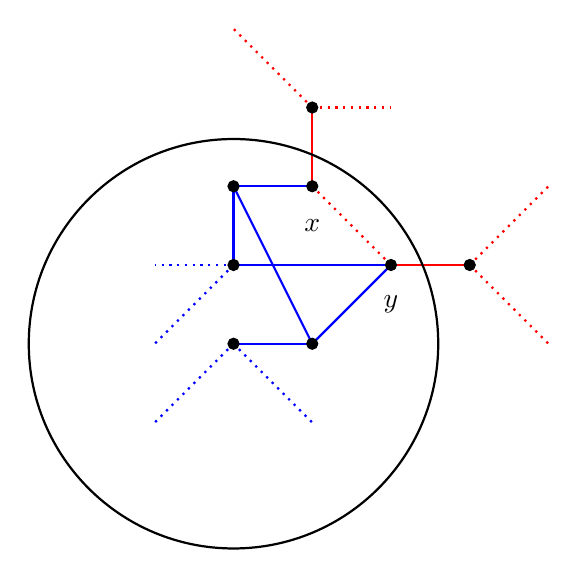
\begin{tikzpicture}
                          \node at (0,0.5,0){$x$};
                          \node at (1,-0.5,0){$y$};
                          \draw[blue, thick] (0, -1) -- (-1,1);
                          \draw[blue, thick] (-1, 0) -- (1,0);
                          \draw[blue, thick] (0, -1) -- (-1,-1);
                          \draw[blue, thick] (0, 1) -- (-1,1);
                          \draw[blue, thick] (-1, 0) -- (-1,1);
                          \draw[blue, thick] (1, 0) -- (0,-1);
                          \draw[red, thick] (1, 0) -- (2,0);
                          \draw[red, thick] (0, 1) -- (0,2);
                          \draw[black, thick] (-1,-1) circle (2.6);
                          \draw[dotted, red, thick] (0, 1) -- (1,0);
                          \draw[dotted, red, thick] (2, 0) -- (3,1);
                          \draw[dotted, red, thick] (2, 0) -- (3,-1);
                          \draw[dotted, red, thick] (0, 2) -- (1,2);
                          \draw[dotted, red, thick] (0, 2) -- (-1,3);
                          \draw[dotted, blue, thick] (-1, 0) -- (-2,0);
                          \draw[dotted, blue, thick] (-1, 0) -- (-2,-1);
                          \draw[dotted, blue, thick] (-1, -1) -- (-2,-2);
                          \draw[dotted, blue, thick] (-1, -1) -- (0,-2);
                          \filldraw[black] (-1,1) circle (2pt);
                          \filldraw[black] (0,-1) circle (2pt);
                          \filldraw[black] (0,1) circle (2pt);
                          \filldraw[black] (1,0) circle (2pt);
                          \filldraw[black] (2,0) circle (2pt);
                          \filldraw[black] (-1,0) circle (2pt);
                          \filldraw[black] (-1,-1) circle (2pt);
                          \filldraw[black] (0,2) circle (2pt);
                      \end{tikzpicture}
                      \caption*{\textcolor{blue}{Xanh}: $M_j-xy$ \\ \textcolor{red}{Đỏ}: $M_p-xy$}
                  \end{figure}


                  Dẫn đến $G$ chứa đồ thị phân chia của $K_5$ hoặc $K_{3,3}$. Vô lý

                  $\Rightarrow \kappa(G) \geq 3$ hay $G$ 3-liên thông.
              \end{proof}
              Tiếp theo, ta sẽ chỉ ra với mọi cặp đỉnh $a,b \in V(G-uv)$, tồn tại một chu trình đi qua chúng.
              Ta sẽ chứng minh qua 3 trường hợp.
              \begin{itemize}
                  \item $\{a,b\} = \{u,v\}$. Vì $\kappa(G) \geq 3$ nên $\nu(G) \geq 4$. Chọn 2 đỉnh $c$ và $d$ bất kỳ trong đồ thị $G-uv$.
                        Không mất tính tổng quát, giả sử $a = u, b = v$. Vì $G$ 3-liên thông nên loại bỏ 2 đỉnh không làm mất tính liên thông của $G$.
                        Nghĩa là khi loại bỏ $v$ và $d$, vẫn còn một đường đi nối giữa $u$ và $c$. Nói cách khác, có một đường đi $P_1$ giữa $u$ và $c$ không đi qua $v$ và $d$.
                        Tương tự, có một đường đi $P_2$ giữa $c$ và $v$ không đi qua $u$ và $d$,
                        một đường đi $P_3$ giữa $v$ và $d$ không đi qua $u$ và $c$,
                        một đường đi $P_4$ giữa $d$ và $u$ không đi qua $v$ và $c$.
                        Khi đó, ta có $u$ và $v$ cùng nằm trên một chu trình $u-P_1-c-P_2-v-P_3-d-P_4-u$.
                  \item Có duy nhất 1 đỉnh trong $\{a,b\}$ là $u$ hoặc $v$. Không mất tính tổng quát, giả sử $a=u$ và $b \neq v$.
                        Chọn bất kỳ điểm $c \neq b$ không trùng $u$ và $v$. Tương tự trường hợp trên,
                        tồn tại một đường đi $P_1$ giữa $u$ và $b$ không đi qua $c$ và $v$,
                        một đường đi $P_2$ giữa $c$ và $b$ không đi qua $u$ và $v$,
                        một đường đi $P_3$ giữa $c$ và $u$ không đi qua $v$ và $b$. Ta lại thu được một chu trình $u-P_1-b-P_2-c-P_3-u$, chu trình này chứa cả $u$ và $b$.
                  \item Cả $a,b$ đều không trùng $u,v$. Lại một lần nữa, tương tự trường hợp trên,
                        tồn tại một đường đi $P_1$ giữa $a,b$ không đi qua $u,v$,
                        một đường đi $P_2$ giữa $b,v$ không đi qua $u,a$,
                        một đường đi $P_3$ giữa $v,a$ không đi qua $u,b$. Ta thu được chu trình $a-P_1-b-P_2-v-P_3-a$ chứa cả $a$ và $b$.
              \end{itemize}
              Từ 3 trường hợp trên, luôn có một chu trình đi qua $a,b$ trong $G-uv$, nên $G-uv$ phải 2-liên thông.

              \begin{tikzpicture}

              \end{tikzpicture}
    \end{enumerate}


    Xét đồ thị $G-uv$ thu được bằng cách bỏ cạnh $uv$ từ $G$

    $G-uv$ là đồ thị phẳng

    $G-uv$ là 2-liên thông, nên tồn tại chu trình đi qua $u$ và $v$.

    \begin{remark}
        Những cạnh chúng tôi vẽ dưới đây là những đường đi trong đồ thị.
    \end{remark}

    \begin{figure}[H]
        \begin{minipage}{0.4\textwidth}
            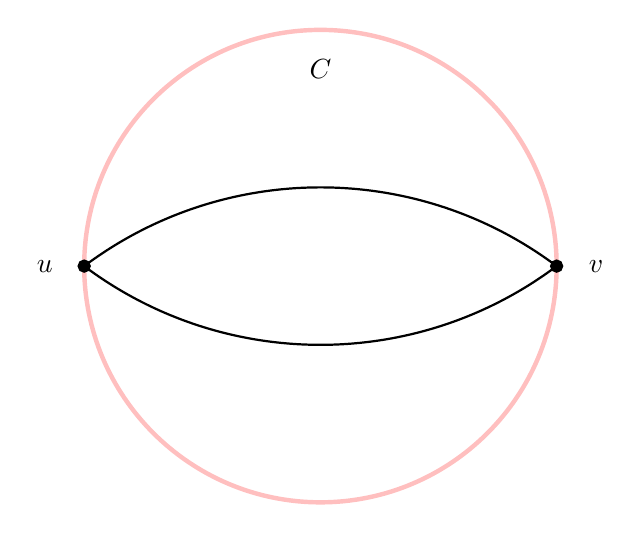
\begin{tikzpicture}
                \draw[pink, ultra thick] (0,0) circle (3);
                \draw[black, thick] (3,0) arc (acos(0.6):180-acos(0.6):5);
                \draw[black, thick] (-3,0) arc (-(180-acos(0.6)):-acos(0.6):5);

                \filldraw[black, thick] (-3,0) circle (2pt);
                \filldraw[black, thick] (3,0) circle (2pt);
                \node at (-3.5,0,0) {$u$};
                \node at (3.5,0,0) {$v$};
                \node at (0,2.5,0) {$C$};
            \end{tikzpicture}
        \end{minipage}
        \hfill
        \begin{minipage}{0.5\textwidth}
            Trong tất cả các chu trình đi qua 2 đỉnh $u,v$ thuộc biểu diễn phẳng của $G-uv$.
            Gọi $C$ là chu trình sao cho số cạnh nằm vùng bên trong nó là lớn nhất.
        \end{minipage}

    \end{figure}

    % \begin{figure}[H]
    %     \begin{minipage}{0.4\textwidth}
    %         \begin{tikzpicture}
    %             \draw[black, thick] (0,0) circle (3);
    %             \filldraw[black, thick] (-3,0) circle (2pt);
    %             \filldraw[black, thick] (3,0) circle (2pt);
    %             \node at (-3.5,0,0) {$u$};
    %             \node at (3.5,0,0) {$v$};
    %             \node at (0,2.5,0) {$C$};
    %         \end{tikzpicture}
    %     \end{minipage}
    %     \hfill
    %     \begin{minipage}{0.5\textwidth}
    %         Có một biểu diễn phẳng của $G$ sao cho $C$ chiếm nhiều diện tích nhất trong tất cả các chu trình chứa $u$ và $v$.
    %     \end{minipage}

    % \end{figure}

    \begin{figure}[H]
        \begin{minipage}{0.4\textwidth}
            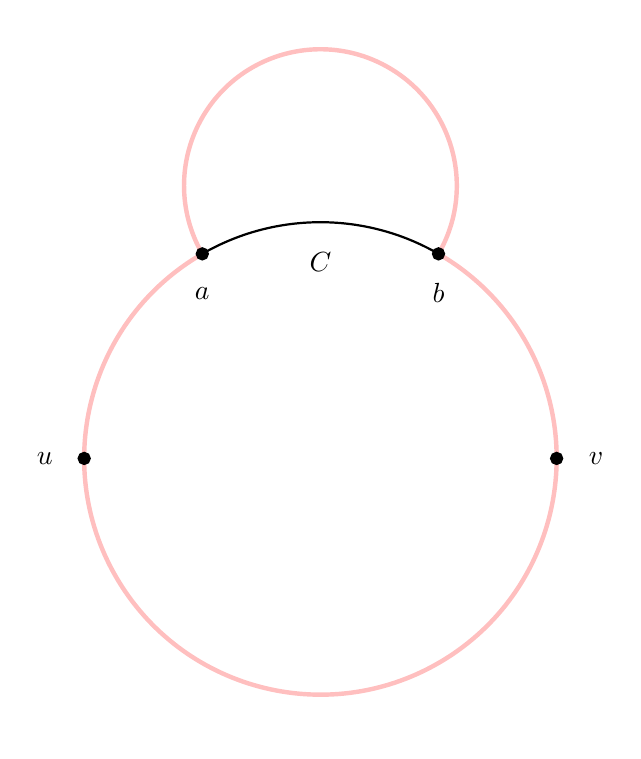
\begin{tikzpicture}
                \draw[pink, ultra thick] (1.5,{sqrt(27/4)}) arc (-30:210:{sqrt(3)});
                \draw[black, thick] (1.5,{sqrt(27/4)}) arc (60:120:3);
                \draw[pink, ultra thick] (-1.5,{sqrt(27/4)}) arc (120:420:3);
                \filldraw[black, thick] (1.5,{sqrt(27/4)}) circle (2pt);
                \filldraw[black, thick] (-1.5,{sqrt(27/4)}) circle (2pt);
                \filldraw[black, thick] (-3,0) circle (2pt);
                \filldraw[black, thick] (3,0) circle (2pt);

                \node at (-1.5,{sqrt(27/4) - 0.5},0) {$a$};
                \node at (1.5,{sqrt(27/4) - 0.5},0) {$b$};
                \node at (-3.5,0,0) {$u$};
                \node at (3.5,0,0) {$v$};
                \node at (0,2.5,0) {$C$};
            \end{tikzpicture}
        \end{minipage}
        \hfill
        \begin{minipage}{0.4\textwidth}
            Với mọi đỉnh $a,b$ nằm trên $C$ mà $a,b$ cùng thuộc một đường đi giữa $u,v$ trên $C$. Ta không thể có đường đi giữa $a,b$ mà nằm ngoài $C$ vì nó sẽ tạo ra chu trình chứa nhiều cạnh ở phía trong hơn $C$ , mâu thuẫn.
        \end{minipage}

    \end{figure}


    \begin{figure}[H]
        \begin{minipage}{0.4\textwidth}
            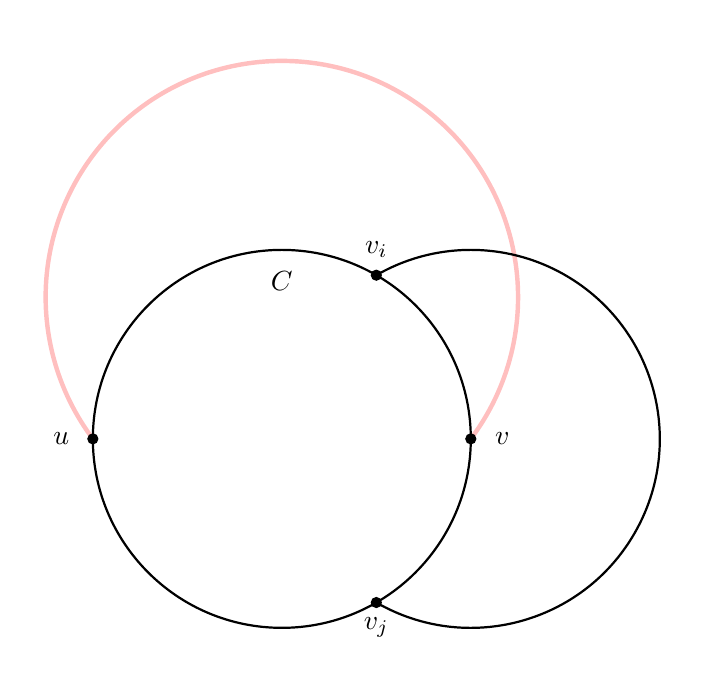
\begin{tikzpicture}[scale = 0.8]
                \draw[black, thick] (0,0) circle (3);
                \draw[pink, ultra thick] (3,0) arc (-acos(3/3.75):180+acos(3/3.75):3.75);
                \draw[black, thick] (1.5,-{sqrt(27/4)}) arc (-120:120:3);

                \filldraw[black, thick] (-3,0) circle (2pt);
                \filldraw[black, thick] (3,0) circle (2pt);
                \filldraw[black, thick] (1.5,{sqrt(27/4)}) circle (2pt);
                \filldraw[black, thick] (1.5,-{sqrt(27/4)}) circle (2pt);
                \node at (1.5,3,0) {$v_i$};
                \node at (1.5,-3,0) {$v_j$};
                \node at (-3.5,0,0) {$u$};
                \node at (3.5,0,0) {$v$};
                \node at (0,2.5,0) {$C$};
            \end{tikzpicture}
        \end{minipage}
        \hfill
        \begin{minipage}{0.4\textwidth}
            Vì $G$ không phẳng nên ta có một đường đi  cắt $uv$ ở phía ngoài của $C$. Gọi đường đi đó là $v_iv_j$ ($v_i,v_j$ nằm trên $C$ và không cùng nằm trên một đường đi giữa $u,v$)
        \end{minipage}
    \end{figure}

    Phía trong của $C$ cũng cần có một phần của đồ thị $G$ cắt đường $v_iv_j$ và $uv$ vẽ từ bên trong của $C$ vì nếu không, ta có thể vẽ đường $v_iv_j$ ở trong và vẽ $uv$ ở bên ngoài hoặc ngược lại để nhận được biểu diễn phẳng của $G$.

    Tương đương, ta có 4 trường hợp tổng quát được miêu tả dưới đây. \\

    \begin{figure}[H]
        \begin{minipage}{0.4\textwidth}
            \begin{tikzpicture}[scale = 0.8]
                \draw[black, thick] (0,0) circle (3);
                \draw[black, thick] (1.5,-{sqrt(27/4)}) arc (-120:120:3);
                \draw[black, thick] ({-sqrt(5)},2) -- ({sqrt(5)},-2);
                \filldraw[black, thick] (-3,0) circle (2pt);
                \filldraw[black, thick] (3,0) circle (2pt);
                \filldraw[black, thick] ({-sqrt(5)},2) circle (2pt);
                \filldraw[black, thick] ({sqrt(5)},-2) circle (2pt);
                \filldraw[black, thick] (1.5,{sqrt(27/4)}) circle (2pt);
                \filldraw[black, thick] (1.5,-{sqrt(27/4)}) circle (2pt);
                \node at (1.5,3,0) {$v_i$};
                \node at (1.5,-3,0) {$v_j$};
                \node at (-3.5,0,0) {$u$};
                \node at (3.5,0,0) {$v$};
                \node at (0,2.5,0) {$C$};
                \node at (2,-4,0) {Trường hợp 1};
            \end{tikzpicture}
        \end{minipage}
        \hfill
        \begin{minipage}{0.4\textwidth}
            \begin{tikzpicture}[scale = 0.8]
                \draw[black, thick] (0,0) circle (3);
                \draw[black, thick] (1.5,-{sqrt(27/4)}) arc (-120:120:3);
                \draw[black, thick] (3,0) arc (acos(0.6):180-acos(0.6):5);
                \draw[black, thick] ({sqrt(5)},-2) -- (-{sqrt(5)},2);
                \filldraw[blue, thick] (-3,0) circle (3pt);
                \filldraw[purple, thick] (3,0) circle (3pt);
                \filldraw[purple, thick] ({-sqrt(5)},2) circle (3pt);
                \filldraw[blue, thick] ({sqrt(5)},-2) circle (3pt);
                \filldraw[blue, thick] (1.5,{sqrt(27/4)}) circle (3pt);
                \filldraw[purple, thick] (1.5,-{sqrt(27/4)}) circle (3pt);
                \node at (1.5,3,0) {$v_i$};
                \node at (1.5,-3,0) {$v_j$};
                \node at (-3.5,0,0) {$u$};
                \node at (3.5,0,0) {$v$};
                \node at (0,2.5,0) {$C$};
                \node at (2,-4,0) {$G$ chứa một đồ thị phân chia của $K_{3,3}$};

            \end{tikzpicture}
        \end{minipage}
    \end{figure}

    \begin{figure}[H]
        \begin{minipage}{0.4\textwidth}
            \begin{tikzpicture}[scale = 0.8]
                \draw[black, thick] (0,0) circle (3);
                \draw[black, thick] (1.5,-{sqrt(27/4)}) arc (-120:120:3);
                \draw[black, thick] (0,0) -- ({sqrt(5)},-2);
                \draw[black, thick] (0,0) -- ({sqrt(5)},2);
                \draw[black, thick] (0,0) -- (-3,0);
                \filldraw[black, thick] (-3,0) circle (2pt);
                \filldraw[black, thick] (3,0) circle (2pt);
                \filldraw[black, thick] (0,0) circle (2pt);
                \filldraw[black, thick] ({sqrt(5)},2) circle (2pt);
                \filldraw[black, thick] ({sqrt(5)},-2) circle (2pt);
                \filldraw[black, thick] (1.5,{sqrt(27/4)}) circle (2pt);
                \filldraw[black, thick] (1.5,-{sqrt(27/4)}) circle (2pt);
                \node at (1.5,3,0) {$v_i$};
                \node at (1.5,-3,0) {$v_j$};
                \node at (-3.5,0,0) {$u$};
                \node at (3.5,0,0) {$v$};
                \node at (0,2.5,0) {$C$};

                \node at (2,-4,0) {Trường hợp 2};
            \end{tikzpicture}
        \end{minipage}
        \hfill
        \begin{minipage}{0.4\textwidth}
            \begin{tikzpicture}[scale = 0.8]
                \draw[black, thick] (0,0) circle (3);
                \draw[black, thick] (1.5,-{sqrt(27/4)}) arc (-120:120:3);
                \draw[black, thick] (3,0) arc (acos(0.6):180-acos(0.6):5);
                \draw[black, thick] (0,0) -- ({sqrt(5)},-2);
                \draw[black, thick] (0,0) -- ({sqrt(5)},2);
                \draw[black, thick] (0,0) -- (-3,0);
                \filldraw[blue, thick] (-3,0) circle (3pt);
                \filldraw[purple, thick] (3,0) circle (3pt);
                \filldraw[purple, thick] (0,0) circle (3pt);
                \filldraw[blue, thick] ({sqrt(5)},2) circle (3pt);
                \filldraw[blue, thick] ({sqrt(5)},-2) circle (3pt);
                \filldraw[black, thick] (1.5,{sqrt(27/4)}) circle (2pt);
                \filldraw[purple, thick] (1.5,-{sqrt(27/4)}) circle (3pt);
                \node at (1.5,3,0) {$v_i$};
                \node at (1.5,-3,0) {$v_j$};
                \node at (-3.5,0,0) {$u$};
                \node at (3.5,0,0) {$v$};
                \node at (0,2.5,0) {$C$};
                \node at (2,-4,0) {$G$ chứa một đồ thị phân chia của $K_{3,3}$};

            \end{tikzpicture}
        \end{minipage}
    \end{figure}

    \begin{figure}[H]
        \begin{minipage}{0.4\textwidth}
            \begin{tikzpicture}[scale = 0.8]
                \draw[black, thick] (0,0) circle (3);
                \draw[black, thick] (1.5,-{sqrt(27/4)}) arc (-120:120:3);
                \draw[black, thick] (3,0) -- (-3,0);
                \draw[black, thick] (1.5,0) -- (1.5,{sqrt(27/4)});
                \draw[black, thick] (-1.5,0) -- (1.5,-{sqrt(27/4)});
                \filldraw[black, thick] (-3,0) circle (2pt);
                \filldraw[black, thick] (3,0) circle (2pt);
                \filldraw[black, thick] (1.5,{sqrt(27/4)}) circle (2pt);
                \filldraw[black, thick] (1.5,-{sqrt(27/4)}) circle (2pt);
                \filldraw[black, thick] (1.5,0) circle (2pt);
                \filldraw[black, thick] (-1.5,0) circle (2pt);
                \node at (1.5,3,0) {$v_i$};
                \node at (1.5,-3,0) {$v_j$};
                \node at (-3.5,0,0) {$u$};
                \node at (3.5,0,0) {$v$};
                \node at (0,2.5,0) {$C$};

                \node at (2,-4,0) {Trường hợp 3};
            \end{tikzpicture}
        \end{minipage}
        \hfill
        \begin{minipage}{0.4\textwidth}
            \begin{tikzpicture}[scale = 0.8]
                \draw[black, thick] (3,0) arc (acos(0.6):180-acos(0.6):5);
                \draw[black, thick] (0,0) circle (3);
                \draw[black, thick] (1.5,-{sqrt(27/4)}) arc (-120:120:3);
                \draw[black, thick] (3,0) -- (-3,0);
                \draw[black, thick] (1.5,0) -- (1.5,{sqrt(27/4)});
                \draw[black, thick] (-1.5,0) -- (1.5,-{sqrt(27/4)});
                \filldraw[purple, thick] (-3,0) circle (3pt);
                \filldraw[blue, thick] (3,0) circle (3pt);
                \filldraw[blue, thick] (1.5,{sqrt(27/4)}) circle (3pt);
                \filldraw[purple, thick] (1.5,-{sqrt(27/4)}) circle (3pt);
                \filldraw[purple, thick] (1.5,0) circle (3pt);
                \filldraw[blue, thick] (-1.5,0) circle (3pt);
                \node at (1.5,3,0) {$v_i$};
                \node at (1.5,-3,0) {$v_j$};
                \node at (-3.5,0,0) {$u$};
                \node at (3.5,0,0) {$v$};
                \node at (0,2.5,0) {$C$};
                \node at (2,-4,0) {$G$ chứa một đồ thị phân chia của $K_{3,3}$};

            \end{tikzpicture}
        \end{minipage}
    \end{figure}


    \begin{figure}[H]
        \begin{minipage}{0.4\textwidth}
            \begin{tikzpicture}[scale = 0.8]
                \draw[black, thick] (0,0) circle (3);
                \draw[black, thick] (1.5,-{sqrt(27/4)}) arc (-120:120:3);
                \draw[black, thick] (3,0) -- (-3,0);
                \draw[black, thick] (0,0) -- (1.5,{sqrt(27/4)});
                \draw[black, thick] (0,0) -- (1.5,-{sqrt(27/4)});
                \filldraw[black, thick] (-3,0) circle (2pt);
                \filldraw[black, thick] (3,0) circle (2pt);
                \filldraw[black, thick] (1.5,{sqrt(27/4)}) circle (2pt);
                \filldraw[black, thick] (1.5,-{sqrt(27/4)}) circle (2pt);
                \filldraw[black, thick] (0,0) circle (2pt);
                \node at (1.5,3,0) {$v_i$};
                \node at (1.5,-3,0) {$v_j$};
                \node at (-3.5,0,0) {$u$};
                \node at (3.5,0,0) {$v$};
                \node at (0,2.5,0) {$C$};

                \node at (2,-4,0) {Trường hợp 4};
            \end{tikzpicture}
        \end{minipage}
        \hfill
        \begin{minipage}{0.4\textwidth}
            \begin{tikzpicture}[scale = 0.8]
                \draw[black, thick] (3,0) arc (acos(0.6):180-acos(0.6):5);
                \draw[black, thick] (0,0) circle (3);
                \draw[black, thick] (1.5,-{sqrt(27/4)}) arc (-120:120:3);
                \draw[black, thick] (3,0) -- (-3,0);
                \draw[black, thick] (0,0) -- (1.5,{sqrt(27/4)});
                \draw[black, thick] (0,0) -- (1.5,-{sqrt(27/4)});
                \filldraw[black, thick] (-3,0) circle (3pt);
                \filldraw[black, thick] (3,0) circle (3pt);
                \filldraw[black, thick] (1.5,{sqrt(27/4)}) circle (3pt);
                \filldraw[black, thick] (1.5,-{sqrt(27/4)}) circle (3pt);
                \filldraw[black, thick] (0,0) circle (3pt);
                \node at (1.5,3,0) {$v_i$};
                \node at (1.5,-3,0) {$v_j$};
                \node at (-3.5,0,0) {$u$};
                \node at (3.5,0,0) {$v$};
                \node at (0,2.5,0) {$C$};
                \node at (2,-4,0) {$G$ chứa một đồ thị phân chia của $K_5$};

            \end{tikzpicture}
        \end{minipage}
    \end{figure}
    \begin{remark}
        $G$ luôn có một đồ thị con là  đồ thị phân chia của $K_5$ hoặc $K_{3,3}$
    \end{remark}
    Kết quả của 4 trường hợp trên đều mâu thuẫn với giả thiết. Từ đây, ta kết luận rằng, không tồn tại đồ thị nào như $G$. Định lý được chứng minh.
\end{proof}
